% Created by tikzDevice version 0.10.1 on 2017-11-27 12:50:33
% !TEX encoding = UTF-8 Unicode
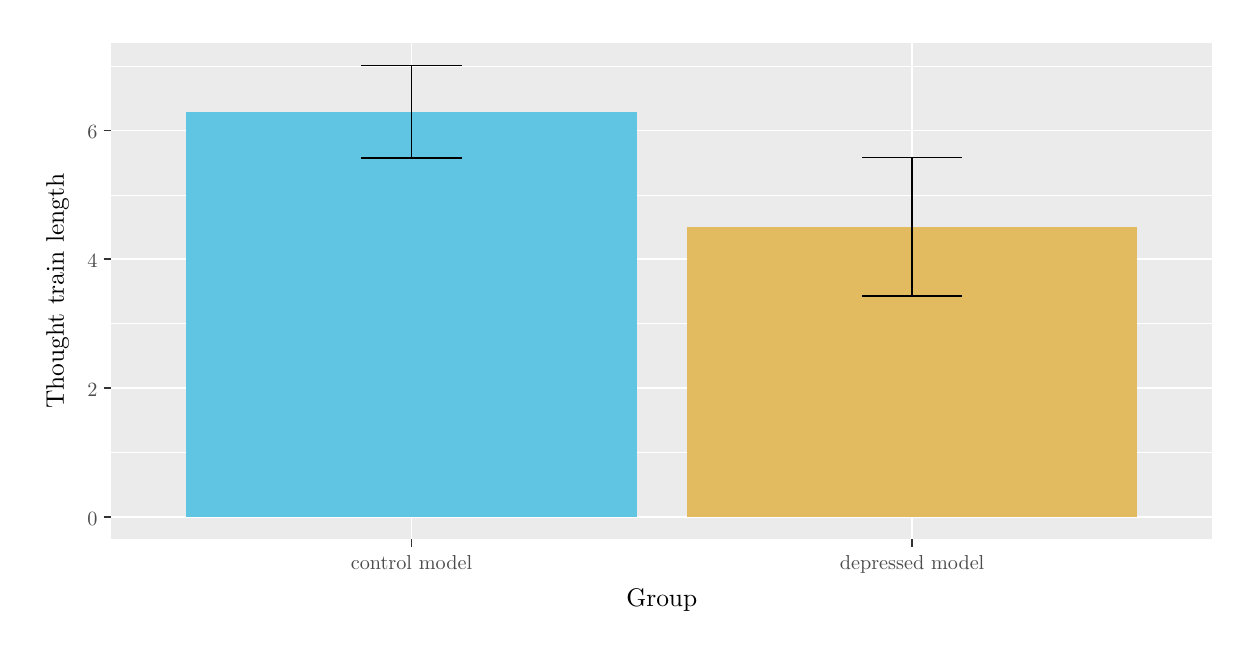
\begin{tikzpicture}[x=1pt,y=1pt]
\definecolor{fillColor}{RGB}{255,255,255}
\path[use as bounding box,fill=fillColor,fill opacity=0.00] (0,0) rectangle (433.62,216.81);
\begin{scope}
\path[clip] (  0.00,  0.00) rectangle (433.62,216.81);
\definecolor{drawColor}{RGB}{255,255,255}
\definecolor{fillColor}{RGB}{255,255,255}

\path[draw=drawColor,line width= 0.6pt,line join=round,line cap=round,fill=fillColor] (  0.00,  0.00) rectangle (433.62,216.81);
\end{scope}
\begin{scope}
\path[clip] ( 30.17, 31.92) rectangle (428.12,211.31);
\definecolor{fillColor}{gray}{0.92}

\path[fill=fillColor] ( 30.17, 31.92) rectangle (428.12,211.31);
\definecolor{drawColor}{RGB}{255,255,255}

\path[draw=drawColor,line width= 0.3pt,line join=round] ( 30.17, 63.33) --
	(428.12, 63.33);

\path[draw=drawColor,line width= 0.3pt,line join=round] ( 30.17,109.85) --
	(428.12,109.85);

\path[draw=drawColor,line width= 0.3pt,line join=round] ( 30.17,156.36) --
	(428.12,156.36);

\path[draw=drawColor,line width= 0.3pt,line join=round] ( 30.17,202.88) --
	(428.12,202.88);

\path[draw=drawColor,line width= 0.6pt,line join=round] ( 30.17, 40.07) --
	(428.12, 40.07);

\path[draw=drawColor,line width= 0.6pt,line join=round] ( 30.17, 86.59) --
	(428.12, 86.59);

\path[draw=drawColor,line width= 0.6pt,line join=round] ( 30.17,133.11) --
	(428.12,133.11);

\path[draw=drawColor,line width= 0.6pt,line join=round] ( 30.17,179.62) --
	(428.12,179.62);

\path[draw=drawColor,line width= 0.6pt,line join=round] (138.70, 31.92) --
	(138.70,211.31);

\path[draw=drawColor,line width= 0.6pt,line join=round] (319.59, 31.92) --
	(319.59,211.31);
\definecolor{fillColor}{RGB}{95,197,226}

\path[fill=fillColor] ( 57.30, 40.07) rectangle (220.10,186.38);
\definecolor{fillColor}{RGB}{226,186,95}

\path[fill=fillColor] (238.19, 40.07) rectangle (400.99,144.83);
\definecolor{drawColor}{RGB}{0,0,0}

\path[draw=drawColor,line width= 0.6pt,line join=round] (120.61,203.16) --
	(156.79,203.16);

\path[draw=drawColor,line width= 0.6pt,line join=round] (138.70,203.16) --
	(138.70,169.61);

\path[draw=drawColor,line width= 0.6pt,line join=round] (120.61,169.61) --
	(156.79,169.61);

\path[draw=drawColor,line width= 0.6pt,line join=round] (301.50,169.90) --
	(337.68,169.90);

\path[draw=drawColor,line width= 0.6pt,line join=round] (319.59,169.90) --
	(319.59,119.77);

\path[draw=drawColor,line width= 0.6pt,line join=round] (301.50,119.77) --
	(337.68,119.77);
\end{scope}
\begin{scope}
\path[clip] (  0.00,  0.00) rectangle (433.62,216.81);
\definecolor{drawColor}{gray}{0.30}

\node[text=drawColor,anchor=base east,inner sep=0pt, outer sep=0pt, scale=  0.73] at ( 25.22, 37.04) {0};

\node[text=drawColor,anchor=base east,inner sep=0pt, outer sep=0pt, scale=  0.73] at ( 25.22, 83.56) {2};

\node[text=drawColor,anchor=base east,inner sep=0pt, outer sep=0pt, scale=  0.73] at ( 25.22,130.07) {4};

\node[text=drawColor,anchor=base east,inner sep=0pt, outer sep=0pt, scale=  0.73] at ( 25.22,176.59) {6};
\end{scope}
\begin{scope}
\path[clip] (  0.00,  0.00) rectangle (433.62,216.81);
\definecolor{drawColor}{gray}{0.20}

\path[draw=drawColor,line width= 0.6pt,line join=round] ( 27.42, 40.07) --
	( 30.17, 40.07);

\path[draw=drawColor,line width= 0.6pt,line join=round] ( 27.42, 86.59) --
	( 30.17, 86.59);

\path[draw=drawColor,line width= 0.6pt,line join=round] ( 27.42,133.11) --
	( 30.17,133.11);

\path[draw=drawColor,line width= 0.6pt,line join=round] ( 27.42,179.62) --
	( 30.17,179.62);
\end{scope}
\begin{scope}
\path[clip] (  0.00,  0.00) rectangle (433.62,216.81);
\definecolor{drawColor}{gray}{0.20}

\path[draw=drawColor,line width= 0.6pt,line join=round] (138.70, 29.17) --
	(138.70, 31.92);

\path[draw=drawColor,line width= 0.6pt,line join=round] (319.59, 29.17) --
	(319.59, 31.92);
\end{scope}
\begin{scope}
\path[clip] (  0.00,  0.00) rectangle (433.62,216.81);
\definecolor{drawColor}{gray}{0.30}

\node[text=drawColor,anchor=base,inner sep=0pt, outer sep=0pt, scale=  0.73] at (138.70, 20.91) {control model};

\node[text=drawColor,anchor=base,inner sep=0pt, outer sep=0pt, scale=  0.73] at (319.59, 20.91) {depressed model};
\end{scope}
\begin{scope}
\path[clip] (  0.00,  0.00) rectangle (433.62,216.81);
\definecolor{drawColor}{RGB}{0,0,0}

\node[text=drawColor,anchor=base,inner sep=0pt, outer sep=0pt, scale=  0.92] at (229.14,  7.83) {Group};
\end{scope}
\begin{scope}
\path[clip] (  0.00,  0.00) rectangle (433.62,216.81);
\definecolor{drawColor}{RGB}{0,0,0}

\node[text=drawColor,rotate= 90.00,anchor=base,inner sep=0pt, outer sep=0pt, scale=  0.92] at ( 13.08,121.61) {Thought train length};
\end{scope}
\end{tikzpicture}
